\documentclass[a4paper]{article}

\usepackage[english]{babel}
\usepackage[utf8]{inputenc}
\usepackage{csquotes}
\usepackage{amsmath, latexsym}
\usepackage{graphicx}
\usepackage{tikz}
\usepackage{listings}
\usepackage{verbatim}
\usepackage{bigints}
\usepackage{float}
\usepackage{titling}
\usepackage[percent]{overpic}
\usepackage[para]{footmisc}
\usepackage[colorinlistoftodos]{todonotes}
\usepackage[style=authoryear,sorting=nty,maxcitenames=1]{biblatex}
\addbibresource{references.bib}

\title{Computation of far-field acoustic pressure from bubble collapse using the Keller-Miksis model}
\author{}
\date{\today}

\begin{document}
\maketitle
\section*{Keller-Miksis model}
In this work we compute the far-field acoustic pressure from bubble collapse using the Keller-Miksis model (\cite{keller1980bubble}, \cite{keller1956damping}).
\subsection*{Governing equation}
\begin{figure}[!h]
    \centering
    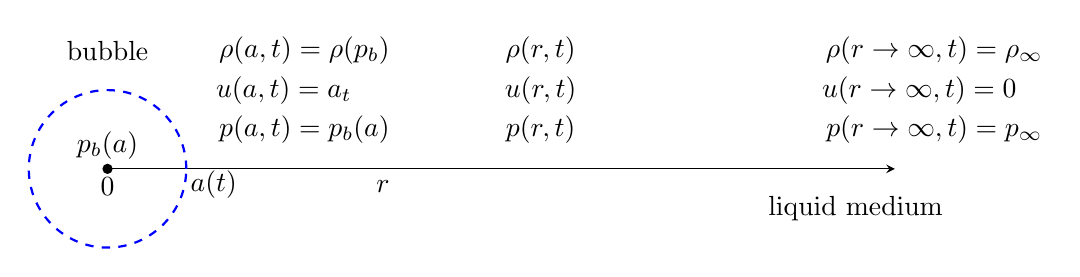
\begin{tikzpicture}
        \draw [-stealth](0, 0) -- (10.0,0);
        \draw [blue, thick, dashed] (0, 0) circle (1);
        \draw [black, thick, fill] (0, 0.0) circle (0.05);
        \draw (0.0, 0.3) node {$p_b(a)$};
        \draw (0.0, 1.5) node {bubble};
        \draw (9.5, -0.5) node {liquid medium};
        \draw (1.35, -0.2) node {$a(t)$};
        \draw (0.0, -0.22) node {$0$};
        \draw (3.5, -0.22) node {$r$};
        \draw (2.5, 1.5) node {$\rho(a, t) = \rho (p_b)$};
        \draw (2.24, 1.0) node {$u(a, t) = a_t$};
        \draw (2.5, 0.5) node {$p(a, t) = p_b(a)$};
        \draw (5.5, 1.5) node {$\rho(r, t)$};
        \draw (5.5, 1.0) node {$u(r, t)$};
        \draw (5.5, 0.5) node {$p(r, t)$};
        \draw (10.5, 1.5) node {$\rho(r\to \infty, t) = \rho_\infty$};
        \draw (10.31, 1.0) node {$u(r\to \infty, t) = 0$};
        \draw (10.5, 0.5) node {$p(r\to \infty, t) = p_{\infty}$};
    \end{tikzpicture}
    \caption{Schematic of a spherical air bubble in liquid medium.}
\end{figure}

A spherical air bubble is placed in an infinite inviscid compressible liquid medium as shown in figure. Assuming spherical symmetry, the mass and momentum conservation equation for the liquid medium is given by
\begin{align}
    \rho_t + \rho_r u + \rho u_r + \frac{2\rho u}{r} & = 0,       \\
    u_t + u u_r + \frac{p_r}{\rho}                   & = 0,       \\
    p                                                & = p(\rho).
\end{align}
Assuming the existence of velocity potential $\phi$, the mass and the momentum conservation equation can be rewritten as
\begin{align}
    \rho_t + \rho_r \phi_r + \rho \phi_{rr} + \frac{2\rho \phi_r}{r} & = 0, \\
    \phi_{rt} + \phi_r \phi_{rr} + \frac{p_r}{\rho}                  & = 0.
\end{align}
We assume the pressure inside the bubble is uniform $p_b$. Assuming adiabatic expansion, the bubble pressure is given as a function of radius $a$,
\begin{equation}
    p_b(a) = k {a}^{-3 \gamma}.
\end{equation}
Where, $k$ is the constant computed from initial radius and pressure and $\gamma$ is the specific heat ratio of the gas. Neglecting surface tension and viscous effects the liquid pressure at bubble wall is same as the pressure inside the bubble. Using continuity, the bubble wall velocity is same as the fluid velocity at bubble radius:
\begin{equation}
    p(a, t) = p_b(a), \;\;\;\;\; \phi_r(a, t) = a_t.
\end{equation}
We can solve the equations $(3) - (6)$ for variables $a, \rho, \phi, p$ given initial conditions.
\subsection*{Simplifications using the Keller-Miksis model}
To solve these equations, we integrate $(5)$ with respect to $r$ from $r$ to infinity.
\begin{equation}
    -\phi_t - \frac{1}{2}\phi_r^2 + \int_{p}^{p_\infty} \rho^{-1} dp = 0.
\end{equation}
We assume $\phi$ tends to zero at $r = \infty$. We differentiate the above equation with respect to $t$ and obtain
\begin{equation}
    -\phi_{tt} - \phi_r\phi_{rt} + c^2\frac{\rho_t}{\rho} = 0.
\end{equation}
Using $(4)$ and replacing $\rho_t$ in $(9)$ we obtain,
\begin{equation}
    \frac{1}{c^2} \phi_{tt} - \phi_{rr} - \frac{2 \phi_r}{r} = \frac{\rho_r \phi_r}{\rho} - \frac{\phi_r \phi_{rt}}{c^2}.
\end{equation}
We omit the right handside in $(10)$ by assuming $c$ is large and $\rho_r$ is small for \textcolor{red}{nearly incompressible fluid}. And obtain the wave equation for $\phi$
\begin{equation}
    \frac{1}{c^2} \phi_{tt} - \phi_{rr} - \frac{2 \phi_r}{r} = 0.
\end{equation}
Assuming $\rho = $ constant in $(8)$ we obtain an equation for pressure
\begin{equation}
    p(r, t) = p_{\infty} - \rho \Big(\phi_t + \frac{1}{2}\phi_r^2 \Big).
\end{equation}
Thus the equations $(4)$ and $(5)$ are simplified to $(11)$ and $(12)$.
\subsection*{Simplified equations}
\begin{figure}[!h]
    \centering
    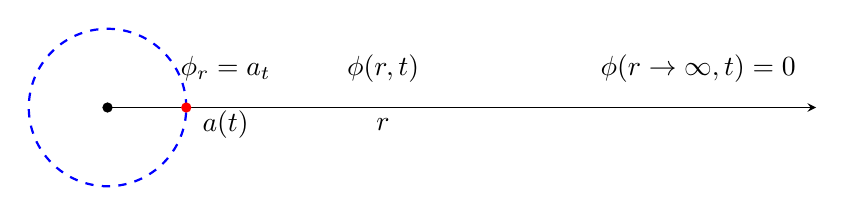
\begin{tikzpicture}
        \draw [-stealth](0, 0) -- (9.0,0);
        \draw [blue, thick, dashed] (0, 0) circle (1);
        \draw [black, thick, fill] (0, 0.0) circle (0.05);
        \draw [red, thick, fill] (1, 0.0) circle (0.05);
        \draw (3.5, 0.5) node {$\phi(r, t)$};
        \draw (3.5, -0.22) node {$r$};
        \draw (1.5, -0.22) node {$a(t)$};
        \draw (1.5, 0.5) node {$\phi_r = a_t$};
        \draw (7.5, 0.5) node {$\phi(r\to \infty, t) = 0$};
    \end{tikzpicture}
\end{figure}
We have to solve the following set of equation for $\phi(r, t)$ and $a(t)$:
\begin{align}
    \frac{1}{c^2}(r \phi)_{tt} - (r \phi)_{rr} & = 0                                                     & r > a(t),   \\
    p_b(a(t)) - p_{\infty}                     & = \rho_{\infty} \Big(\phi_t + \frac{1}{2}\phi_r^2\Bigg) & r = a(t),   \\
    \phi_r                                     & = a_t                                                   & r = a(t),   \\
    \phi                                       & = 0                                                     & r = \infty, \\
    \phi(r, 0)                                 & = 0                                                     & r > a(t),   \\
    \phi_t(r, 0)                               & = 0                                                     & r > a(t),   \\
    a(0)                                       & = a_0,                                                                \\
    a_t(0)                                     & = a_{t0}.
\end{align}

\subsection*{Solution}
A nonlinear second-order ordinary differential equation for $a(t)$ can be obatined by using the solution of wave equation $\phi = f(t - (r - a_0)/c)/r$
\begin{equation}
    \Bigg( 1 - \frac{\Dot{a}}{c} \Bigg)a \Ddot{a} + \frac{3}{2} \Bigg(1 - \frac{\Dot{a}}{3c} \Bigg)\Dot{a}^2 = \frac{1}{\rho_\infty} \Bigg( 1 + \frac{\Dot{a}}{c} + \frac{a}{c}\frac{d}{dt}\Bigg)(p_b - p_\infty).
\end{equation}
Where,  $p$ is the bubble wall pressure given by
\begin{equation}
    p_b = p_{0} \Bigg( \frac{a_0}{a} \Bigg)^{3 \gamma}, \;\;\; \gamma = 1.4.
\end{equation}
The far-field pressure is given by
\begin{equation}
    p(r, t) - p_{\infty} = \rho_\infty\Big( -\frac{f'}{r} -\frac{f^2}{2r^4} - \frac{1}{2c} \Big( \frac{f^{'2}}{cr^2} + \frac{2ff'}{r^3}   \Big) \Big ).
\end{equation}
Where
\begin{equation}
    f = -a^2 a_t + \frac{a^2}{c}\Big( \frac{a_t^2}{2} + \frac{(p_b - p_\infty)}{\rho_\infty}\Big)
\end{equation}
and
\begin{equation}
    f' = -a\Big( \frac{a_t^2}{2} + \frac{(p_b - p_\infty)}{\rho_\infty} \Big).
\end{equation}
Where $a$ is evaluated at retarded time $\tau \approx t - r/c$.
\subsection*{Results}
We solve the evolution of bubble radius for the following simulation parameters
\begin{figure}[!h]
    \centering
    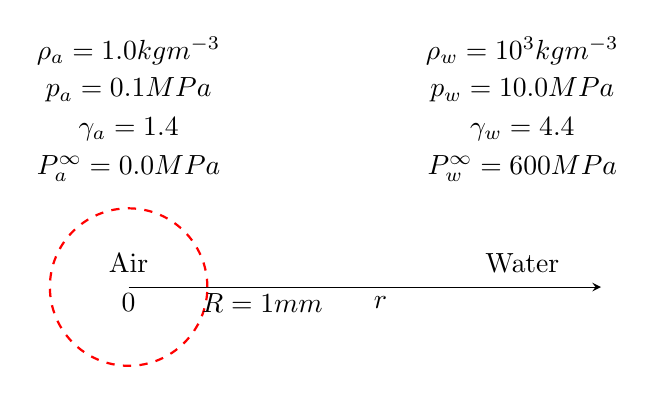
\begin{tikzpicture}
        \draw (0, 0) -- (6.0,0)[-stealth];
        \draw [red, thick, dashed] (0, 0) circle (1);
        \draw (1.7, -0.2) node {$R = 1mm$};
        \draw (3.2, -0.2) node {$r$};
        \draw (0.0, 0.3) node {Air};
        \draw (5.0, 0.3) node {Water};
        \draw (0.0, -0.2) node {0};
        \draw (0.0, 3.0) node {$\rho_a = 1.0 kgm^{-3}$};
        \draw (0.0, 2.5) node {$p_a = 0.1 MPa$};
        \draw (0.0, 2.0) node {$\gamma_a = 1.4$};
        \draw (0.0, 1.5) node {$P^{\infty}_a = 0.0 MPa$};
        \draw (5.0, 3.0) node {$\rho_w = 10^3 kgm^{-3}$};
        \draw (5.0, 2.5) node {$p_w = 10.0 MPa$};
        \draw (5.0, 2.0) node {$\gamma_w = 4.4$};
        \draw (5.0, 1.5) node {$P^{\infty}_w = 600 MPa$};
    \end{tikzpicture}
    \caption{Schematic of air bubble in water medium with the initial conditions.}
\end{figure}
We scale the pressure, density and length using the following scales
\begin{equation}
    \bar{p} = 10^5Pa, \;\;\;\; \bar{\rho} = 1000 kgm^{-3}, \;\;\;\; \bar{l} = 10^{-3} m.
\end{equation}

\begin{figure}[!h]
    \centering
    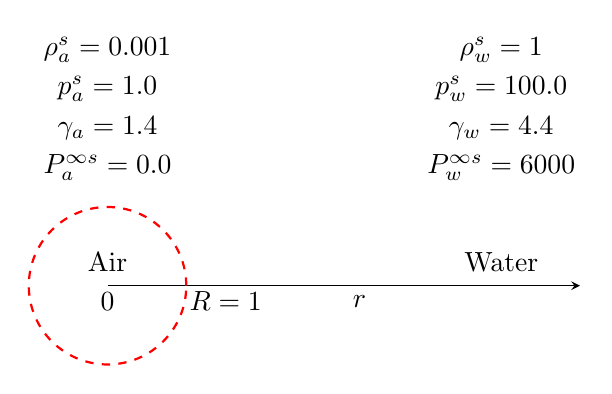
\begin{tikzpicture}
        \draw (0, 0) -- (6.0,0)[-stealth];
        \draw [red, thick, dashed] (0, 0) circle (1);
        \draw (1.5, -0.2) node {$R = 1$};
        \draw (3.2, -0.2) node {$r$};
        \draw (0.0, 0.3) node {Air};
        \draw (5.0, 0.3) node {Water};
        \draw (0.0, -0.2) node {0};
        \draw (0.0, 3.0) node {$\rho_a^s = 0.001$};
        \draw (0.0, 2.5) node {$p_a^s = 1.0 $};
        \draw (0.0, 2.0) node {$\gamma_a = 1.4$};
        \draw (0.0, 1.5) node {$P^{\infty s}_a = 0.0$};

        \draw (5.0, 3.0) node {$\rho_w^s = 1$};
        \draw (5.0, 2.5) node {$p_w^s = 100.0 $};
        \draw (5.0, 2.0) node {$\gamma_w = 4.4$};
        \draw (5.0, 1.5) node {$P^{\infty s}_w = 6000 $};
    \end{tikzpicture}
    \caption{Schematic of air bubble in water medium with the scaled simulation parameters.}
\end{figure}
\begin{figure}[!h]
    \centering
    \includegraphics[scale=0.6]{images/radius.png}
    \caption{Time evolution of the bubble radius.}
\end{figure}
\begin{figure}[!h]
    \centering
    \includegraphics[scale=0.6]{images/pressure.png}
    \caption{The far-field pressure is computed at the observer point $r = 100R$ using the Keller-Kolodner model and compared with the numerical solution of the compressible multiphase Euler equations.
    }
\end{figure}

\printbibliography
\end{document}